\subsection{Visual Based Localization}

\label{sec:intro}

\begin{frame}{Image retrieval}
	
	Image retrieval for Visual Based Localization (\textbf{VBL}): recover the most visually relevant geo-referenced images in a known database.
			
	\begin{minipage}[c]{0.3\linewidth}
		\centering
		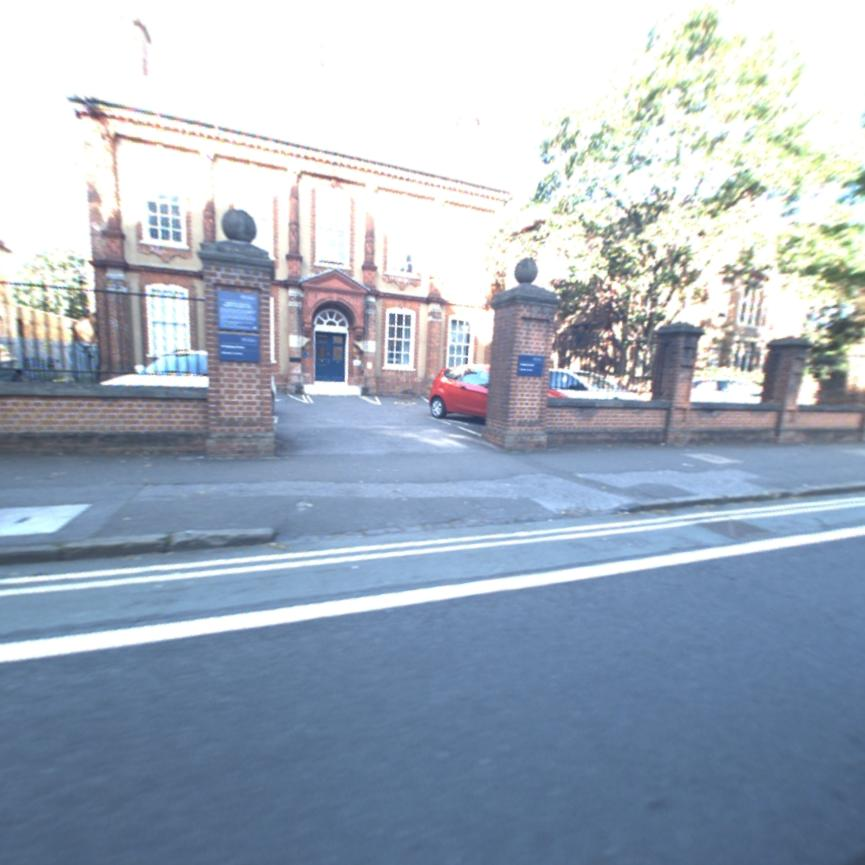
\includegraphics[width=0.6\linewidth]{images/intro/query.jpg}
		
		\textbf{Input query}
	\end{minipage}
	\hfill $\rightarrow$ \hfill 
	\begin{minipage}[c]{0.5\linewidth}
		\centering
	
		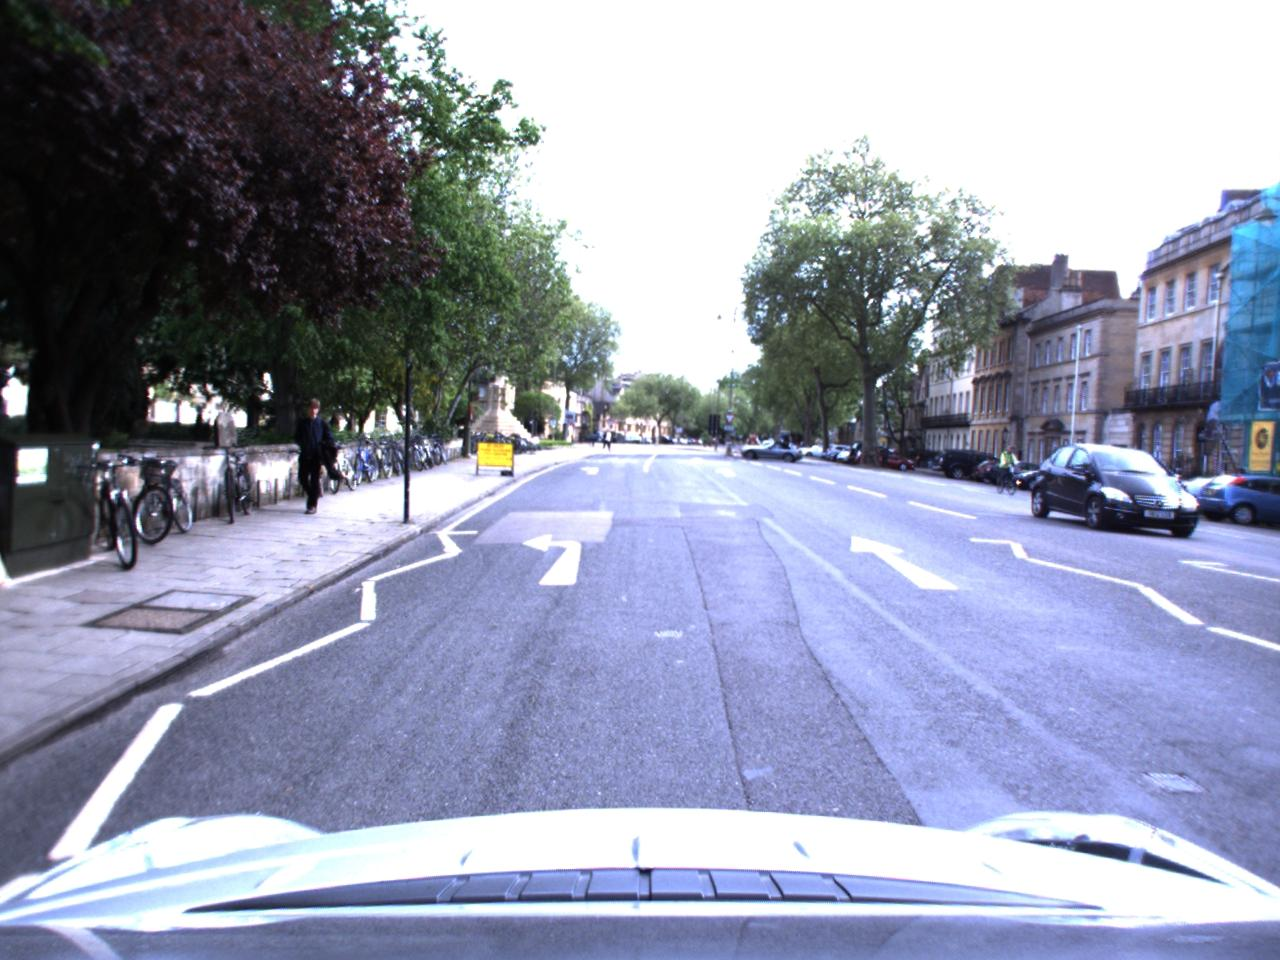
\includegraphics[width=0.3\linewidth]{images/intro/1.jpg} \hspace{0.1cm}
		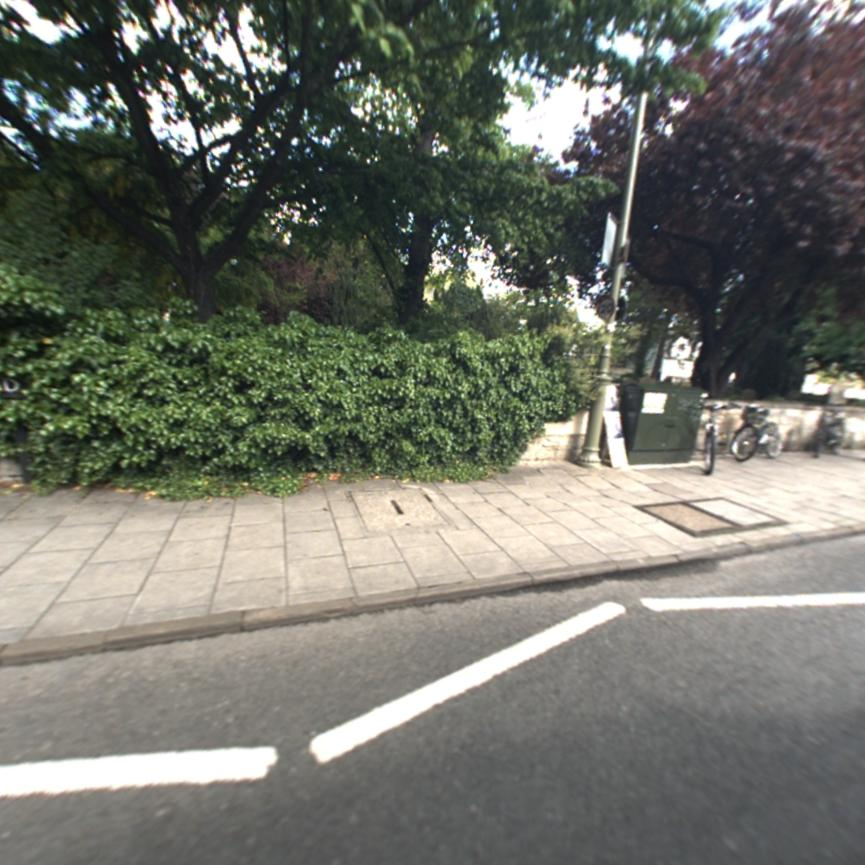
\includegraphics[width=0.3\linewidth]{images/intro/2.jpg} \hspace{0.1cm}
		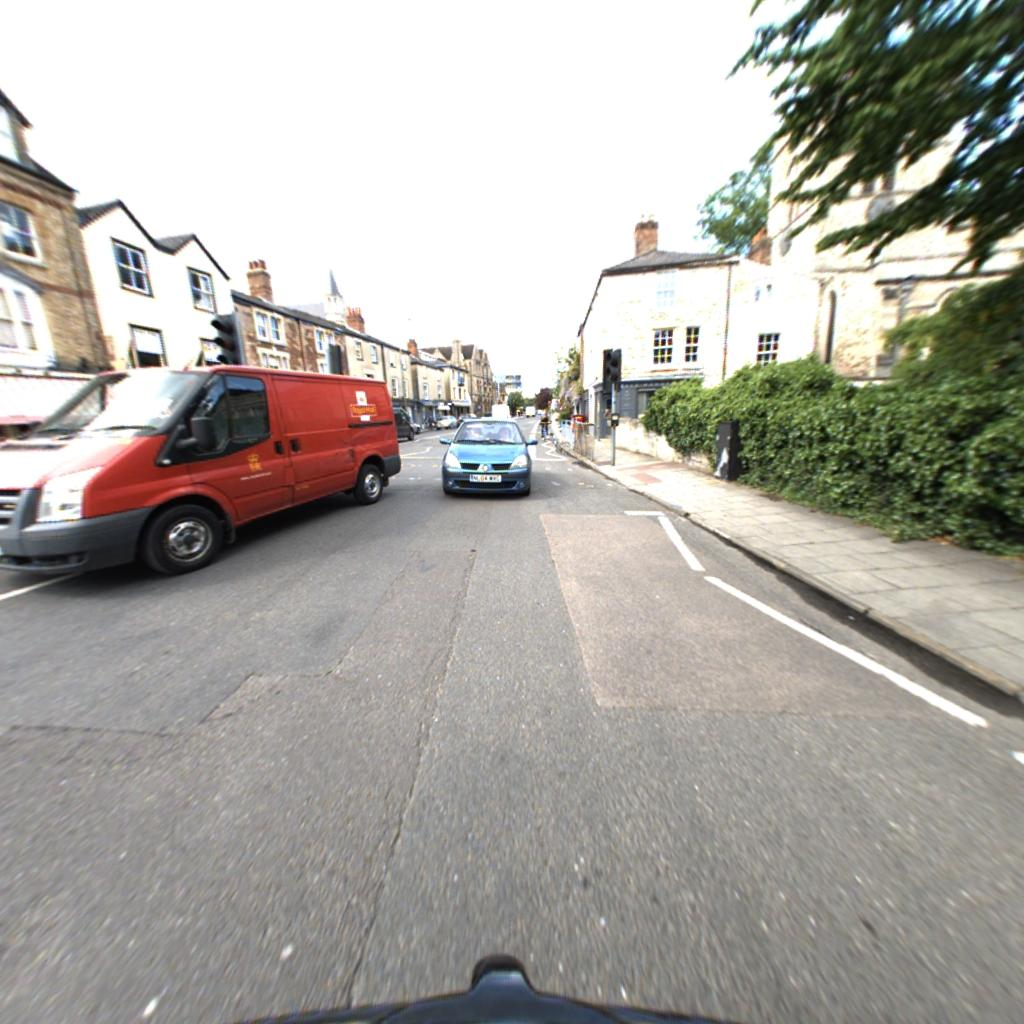
\includegraphics[width=0.3\linewidth]{images/intro/3.jpg} \hspace{0.1cm}
		
		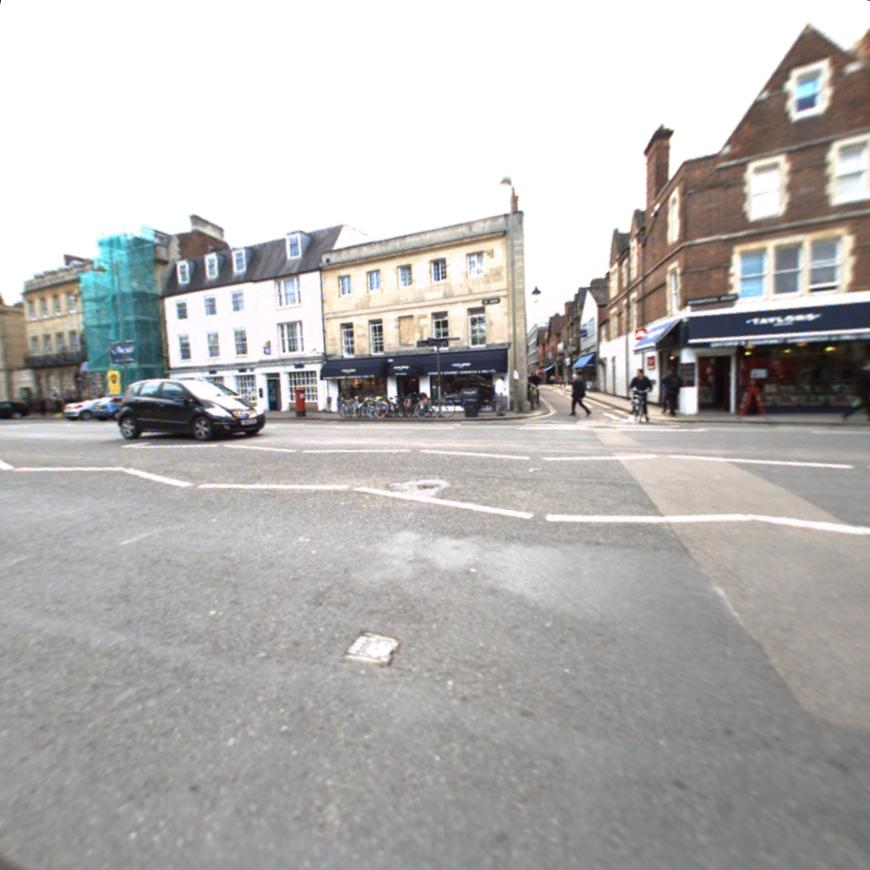
\includegraphics[width=0.3\linewidth]{images/intro/4.jpg} \hspace{0.1cm}
		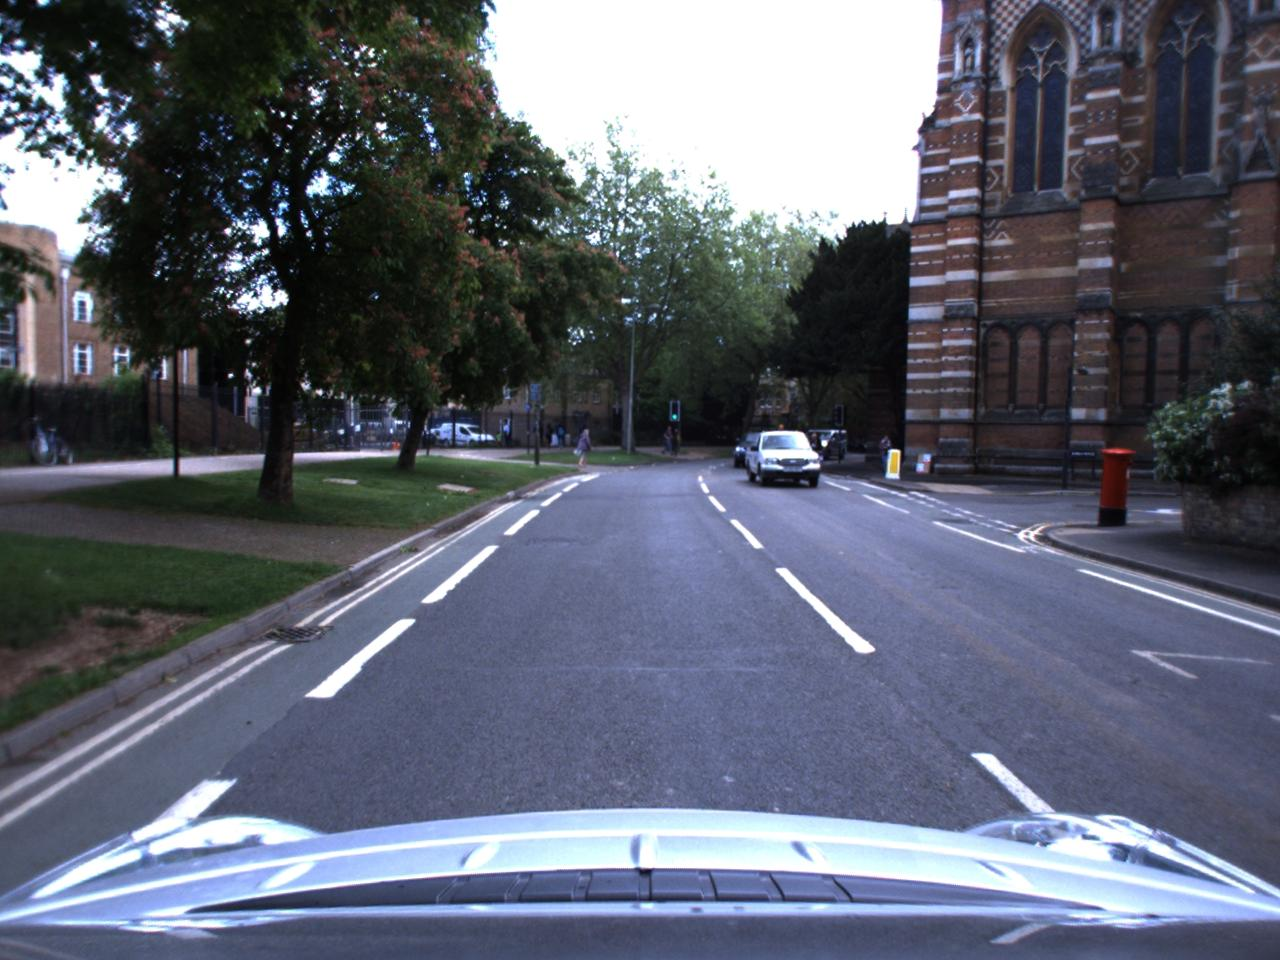
\includegraphics[width=0.3\linewidth]{images/intro/5.jpg} \hspace{0.1cm}
		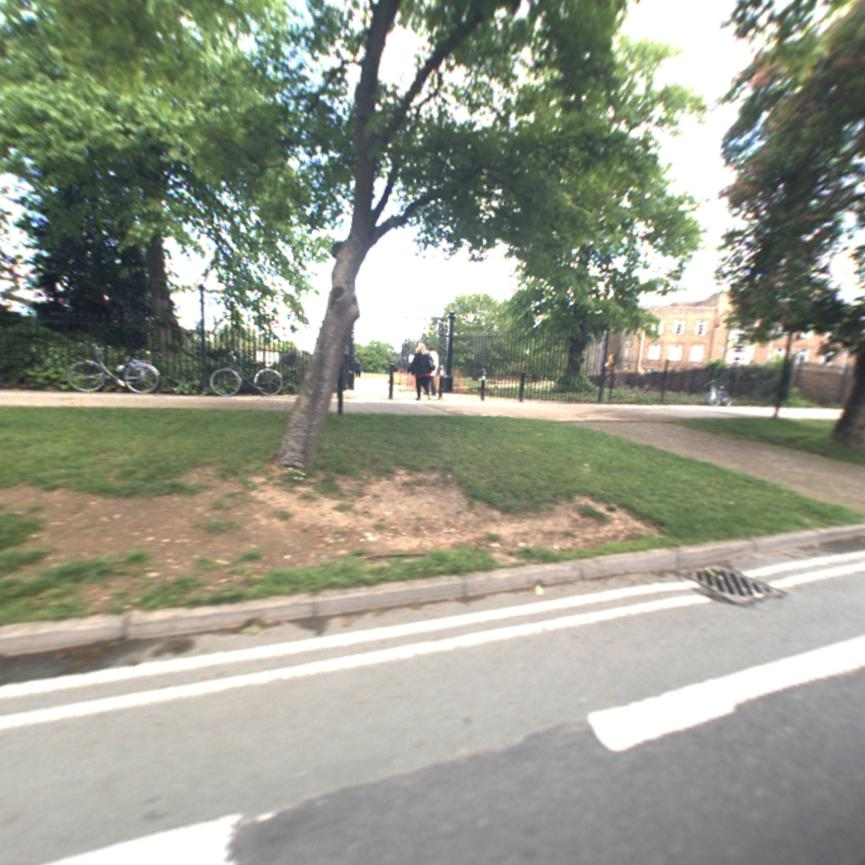
\includegraphics[width=0.3\linewidth]{images/intro/6.jpg} \hspace{0.1cm}
		
		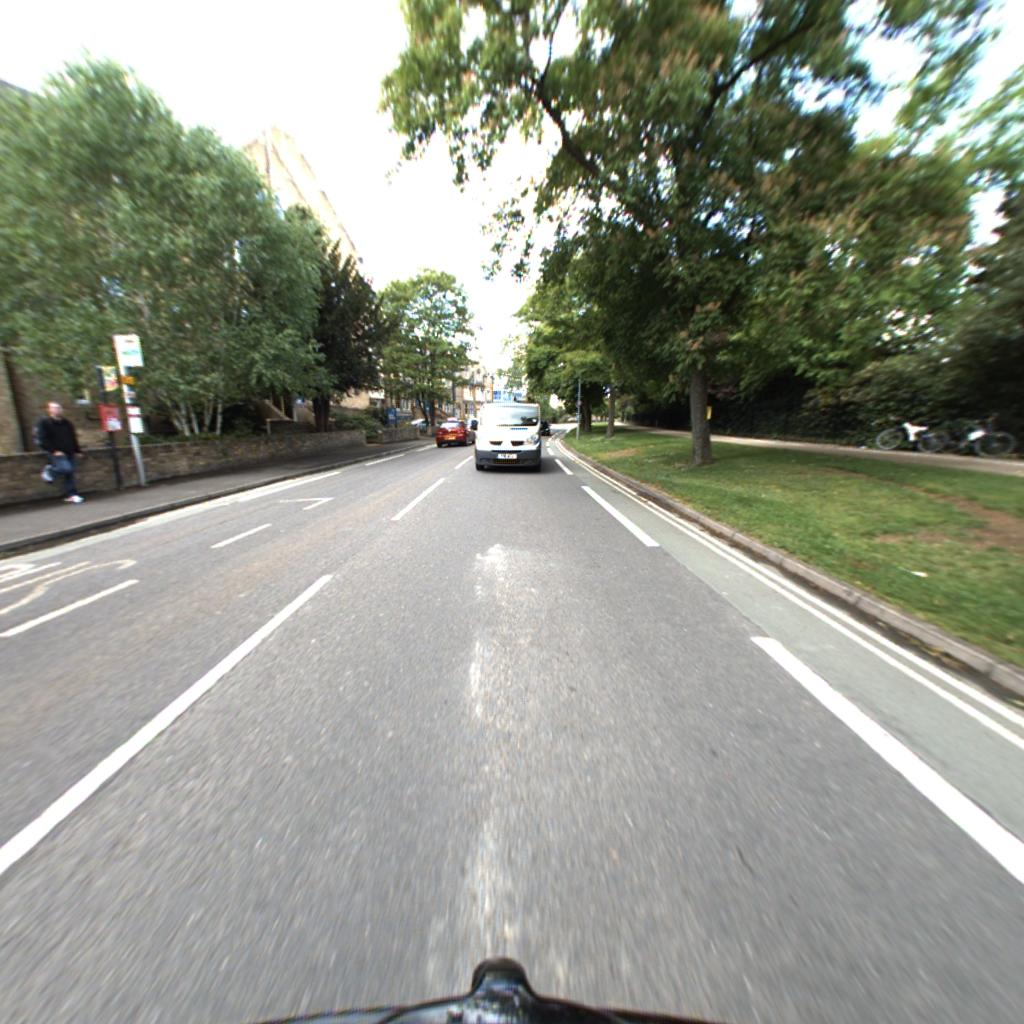
\includegraphics[width=0.3\linewidth]{images/intro/7.jpg} \hspace{0.1cm}
		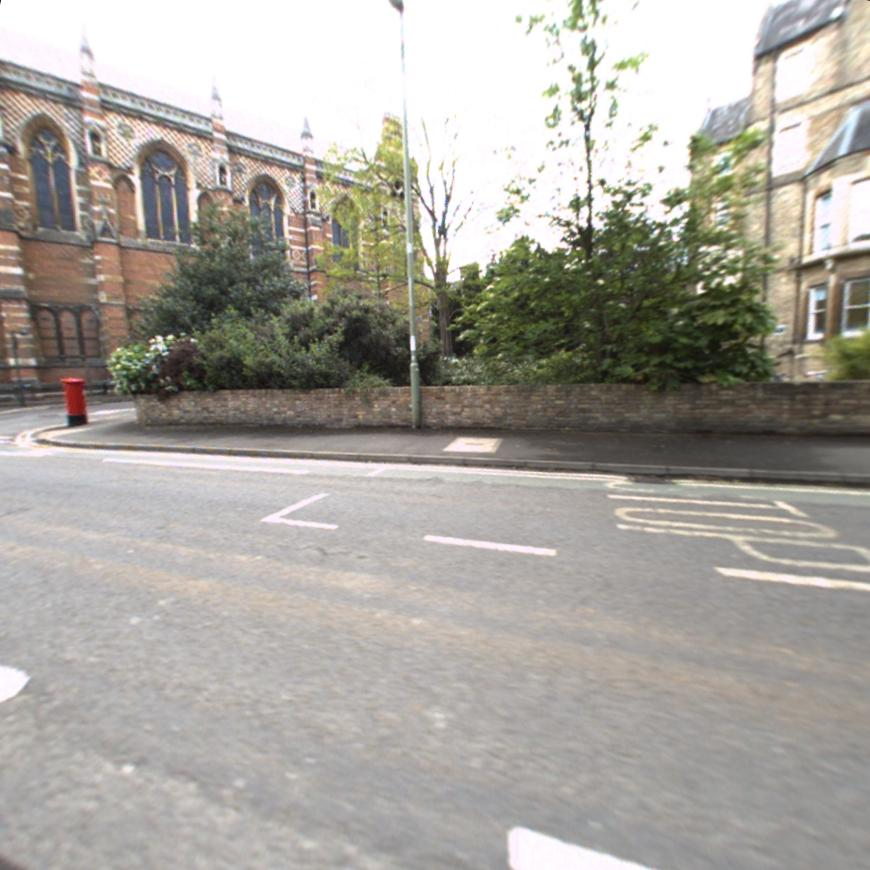
\includegraphics[width=0.3\linewidth]{images/intro/8.jpg}\hspace{0.1cm}
		...
		
		\textbf{Database	of geolocalized images}
	\end{minipage}

\end{frame}

\begin{frame}{Roadmap}

	We want to create an indirect method to localize a query within a set of \textbf{geolocalized} RGB-D images. The considered pipeline will be:
	
	\begin{figure}
		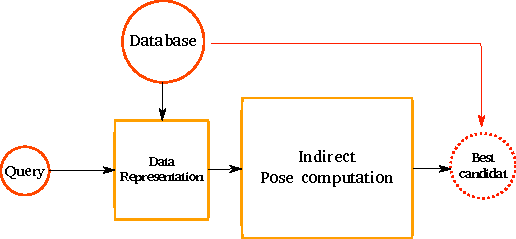
\includegraphics{vect/keys_comp_indirect.pdf}		
		\caption{Visual Based Localization (VBL) pipeline}
	\end{figure}		
		
\end{frame}

\begin{frame}{Data representation}
	We first focus our work on creating a robust data representation. Research on state of the art shown that CNN are the best choice~\cite{Arandjelovic2017}.
	
	\begin{block}{Encoder for data representation}
		\begin{figure}[c]
			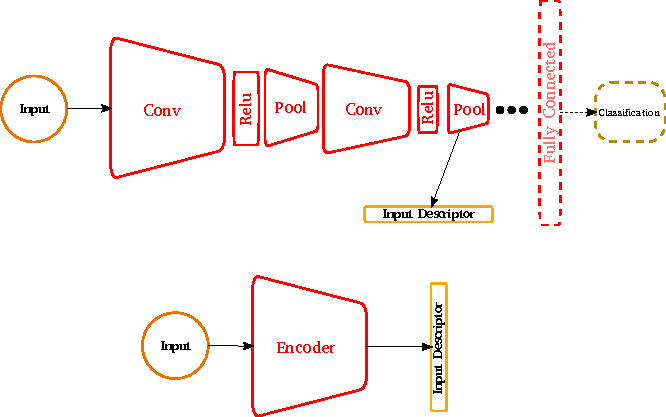
\includegraphics[width=0.75\linewidth]{vect/encodeur.pdf}					
		\end{figure}
	\end{block}
	
\end{frame}

